%!TEX root = ../article.tex

% Conclusion
\section{Grundlagen}
\label{sec:grundlagen}

\subsection{Marching Cubes}
\label{subsec:marchingCubes}
Der Marching Cubes Algorithmus wurde entwickelt um gemessene Voxeldaten bei einem medizinischen Scan darzustellen. Beim Marching Cubes Algorithmus werden immer Tupel aus acht Voxeln gebildet, die in kubischer Form angeordnet sind. Bei diesen wird geprüft, ob diese gefüllt sind. Um die gefüllten von den nicht gefüllten Voxeln durch Flächen zu trennen, werden für die jeweilige Konstellation die entsprechenden Vertices aus einer vorgefertigten Lookup-Table erzeugt (siehe Abbildung 1). Dabei liegt ein Vertex immer auf der Kante zwischen den Mittelpunkten eines gefüllten und eines nicht gefüllten Voxels (siehe Abbildung 2). Zur genaueren Repräsentation des gescannten Objektes werden diese Vertices auf der jeweiligen Kante so verschoben, dass ihre Position auf den gemessenen Eintrittspunkten in das gescannte Objekt liegen (siehe Abbildung 3). Sind keine Informationen über die originalen Schnittpunkte vorhanden, so werden die Vertices meist auf der Mitte der Kante platziert. \cite{lorensen1987marching} \cite{iomc} \cite{mc02}

\begin{figure}[H]
			\centering
			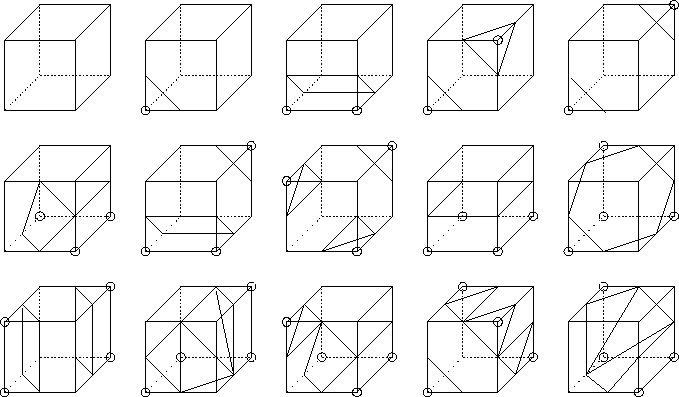
\includegraphics[width=0.5\textwidth]{figures/MarchingCubesPossibilities}
			\caption[Möglichkeiten für MarchingCubes\cite{mc02}]{Möglichkeiten für Marching Cubes \label{MarchingCubesPossibilities}}
		\end{figure}
		
		\begin{minipage}[t]{0.22\textwidth}
			\begin{figure}[H]
			\centering
			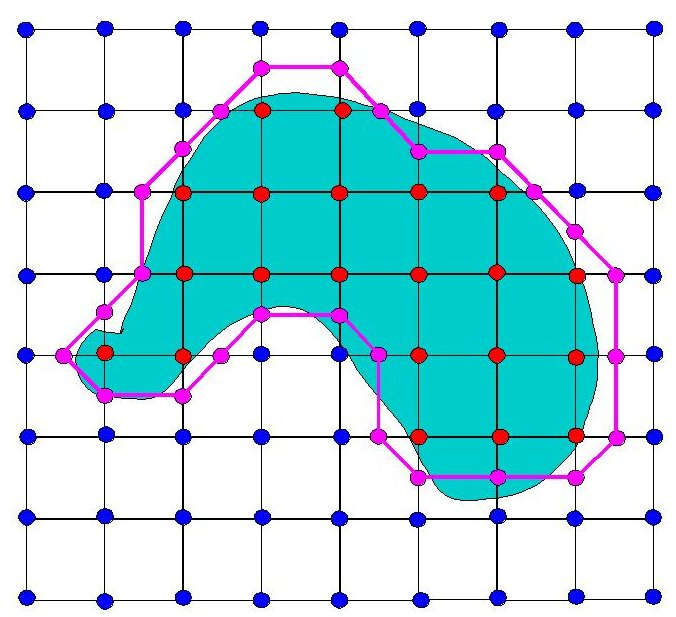
\includegraphics[width=0.98\textwidth]{figures/VerschiebenBeiMarchingCubes1}
			\caption[Marching Cubes Verschiebung (vorher)\cite{iomc}]{Verschiebung bei Marching Cubes (vorher) \label{VerschiebenBeiMarchingCubes1}}
			\end{figure}
			\end{minipage}
			\begin{minipage}[t]{0.22\textwidth}
			\begin{figure}[H]
			\centering
			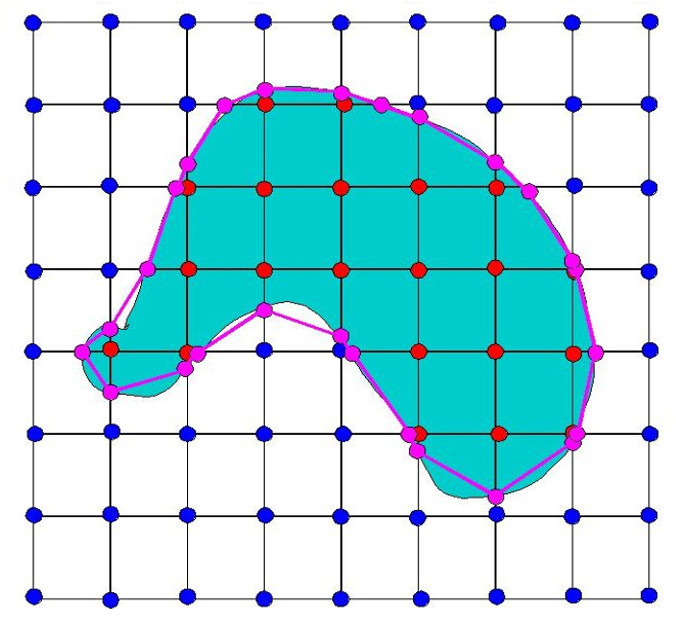
\includegraphics[width=0.98\textwidth]{figures/VerschiebenBeiMarchingCubes2}
			\caption[Marching Cubes Verschiebung (nacher)\cite{iomc}]{Verschiebung bei Marching Cubes (nachher) \label{VerschiebenBeiMarchingCubes2}}
			\end{figure}
			\end{minipage}

\subsection{Material-Interpolation in Marching cubes}
\label{subsec:materialInterpolation}
Eine Methode um Voxel mit jeweils einem Material mit fließenden Übergängen in der Materialdarstellung zwischen unterschiedlichen Materialien zu rendern ist es, den Vertices beim Erstellen jeweils den gefüllten Voxel an der Kante, auf der sie liegen, als primären Voxel zuzuweisen. Somit wird dem jeweiligen Vertex auch das Material des Voxels zugeordnet. Um die Materialien zu interpolieren, werden jedem Vertex die Materialindizes aller Vertices des zu rendernden Polygons und eine Gewichtung für jeden Vertex im Polygon zugewiesen. Durch die Interpolation dieser Werte wird im Polygon bestimmt, welches Material wo gerendert wird. \cite{iomt}

\begin{figure}[H]
			\centering
			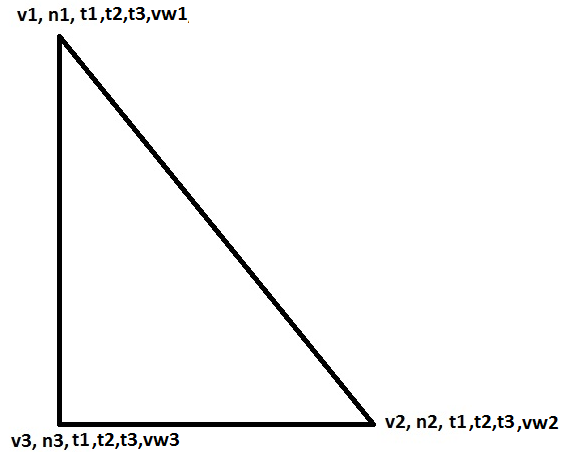
\includegraphics[width=0.3\textwidth]{figures/triangleCorrected}
			\caption[Polygon mit zusätzlichen Werten zur Interpolation\cite{iomt}]{Polygon mit zusätzlichen Werten zur Interpolation: (v*) Vertex Position, (n*) Normale, (t1, t2 und t3) Materialien der drei Richtungen, (vw*) Gewicht der Materialien am Vertex \label{PolygonMitZusatzWerten}}
			\end{figure}

\subsection{Triplanares Mapping}
\label{subsec:triplanaresMapping}
Um zweidimensionale Texturen ohne Verzerrungen und ohne unterschiedliche Detailgrade auf ein beliebiges Objekt zu mappen, wird Triplanares Mapping verwendet. Hierzu werden die dreidimensionalen Positionen innerhalb des Objektes in die drei planaren Projektionen aus Richtung der Hauptachsen aufgeteilt. Für die drei so erzeugten zweidimensionalen Positionen wird jeweils die Farbe aus der Textur gesucht. Die drei so erhaltenen Werte werden anhand der Werte der Normalen des Polygons an der jeweiligen Position gemischt. \cite{tpm}



